\pdfoptionpdfminorversion=5
\documentclass[9pt,hyperref={pdfpagelabels=false}]{beamer}
\setbeameroption{show notes}
\mode<presentation> {
    \usetheme{HHUD}
    \setbeamercovered{invisible}
}
\usepackage[ngerman]{babel}
\usepackage[utf8x]{inputenc}
\usepackage{times}
\usepackage[T1]{fontenc}
\usepackage{amsmath}
\usepackage{subfigure}
\usepackage{graphicx}
\usepackage{hyperref}
\usepackage{xmpmulti}
\usepackage{multicol}
\usepackage{appendixnumberbeamer}
\usepackage{tabularx}
\usepackage{listings}

% background image
\usebackgroundtemplate{
\includegraphics[width=\paperwidth]{fig/background}}
% commands for low and high decoration in frame foot
\newcommand{\footdecorationlow}{\usebackgroundtemplate{
\includegraphics[width=\paperwidth]{fig/background_small}}}
\newcommand{\footdecorationhigh}{\usebackgroundtemplate{
\includegraphics[width=\paperwidth]{fig/background}}}

% Fix build errors on debian (http://bugs.debian.org/cgi-bin/bugreport.cgi?bug=452333)
\providecommand \thispdfpagelabel[1]{} {}

%% Die folgenden Zeilen können auskommentiert werden, um vor jedem Kapitel eine Gliederungsfolie einzufügen
% \AtBeginSection[] {
%   \footdecorationhigh
%   \begin{frame}<beamer>
%     \thispagestyle{empty}
%     \frametitle{Gliederung}
%     \vspace{-5mm}
%     \tableofcontents[currentsection]
%   \end{frame}
%   \footdecorationlow
% }

% % % % % % % % % %  CHANGE TOPIC AND AUTHOR INFORMATION HERE % % % % % % % % %
\newcommand{\abschluss}{Bachelor}                              % HIER UNZUTREFFENDES LÖSCHEN
\title{\abschluss{}arbeit:\\Verteiltes Veranstaltungsmanagement mit einer mobilen Webanwendung}                      % HIER DEN TITEL DER ARBEIT EINTRAGEN
\author{Christian Meter}                                                       % HIER DEN NAMEN UND VORNAMEN EINTRAGEN
\date{10.10.2013}                                                                % HIER DAS PRÄSENTATIONSDATUM EINTRAGEN
% % % % % % % % % % % % % % % % % % % % % % % % % % % % % % % % % % % % % % % %
\institute{Institut für Informatik\\Heinrich-Heine-Universität Düsseldorf}
\subject{Informatik}

%
% Hier beginnt das Dokument
%
\begin{document}

  \footdecorationhigh
  \begin{frame}
    \thispagestyle{empty}
    \titlepage
  \end{frame}

  \begin{frame}
    \thispagestyle{empty}
    \frametitle{Gliederung}
    \vspace{-5mm}
    \tableofcontents
  \end{frame}
  \footdecorationlow

  % % % % % % % % % % Ab hier werden die LaTeX-Dateien der einzelnen Abschnitte eingefügt % % % % % % % % % %

  \section{Einleitung}

\begin{frame}
	\frametitle{Problembeschreibung}
	\begin{itemize}
		\item<1-> 1 Veranstaltung
		\item<2-> 89 ehrenamtliche Helfer, zunächst deutschlandweit verteilt
		\item<3-> 3500 Teilnehmer
		\item<4-> Verschiedene Aufgabenverteilung
		\begin{enumerate}
			\item<4-> Anmeldungen bearbeiten
			\item<4-> Helfer verwalten
			\item<4-> Statistiken erstellen und auswerten
			\item<4-> \dots
		\end{enumerate}
	\end{itemize}

	\begin{block}{Wie soll man produktiv zusammenarbeiten?}<5->
		Viele Personen, verschiedene Standorte, Betriebssysteme, usw.
	\end{block}
\end{frame}

%%%%%%%%%%%%%%%%%%%%%%%%%%%%%%%%%%%%%%%%%%%%%%%%%%%%%%%%%%%%%%%%%%%%%%%%%%%%%%%%%%%%%%

\begin{frame}
	\frametitle{Was wird benötigt?}
	\begin{figure}
		\includegraphics<2>[width=0.8\textwidth]{fig/aufbau_app_1.pdf}
		\includegraphics<3>[width=0.8\textwidth]{fig/aufbau_app_2.pdf}
		\includegraphics<4>[width=0.8\textwidth]{fig/aufbau_app_3.pdf}
		\includegraphics<5>[width=0.8\textwidth]{fig/aufbau_app_4.pdf}
		\includegraphics<6>[width=0.8\textwidth]{fig/aufbau_app_5.pdf}
		\includegraphics<7>[width=0.8\textwidth]{fig/aufbau_app_6.pdf}
		\includegraphics<8>[width=0.8\textwidth]{fig/aufbau_app.pdf}
	\end{figure}
\end{frame}

  \section{Webanwendung}

\begin{frame}
	\frametitle{Die Meißner-App}
    


\end{frame}
  
  \section{Analyse und Auswertung}

\begin{frame}{Benchmark WebServer}
	\begin{figure}
		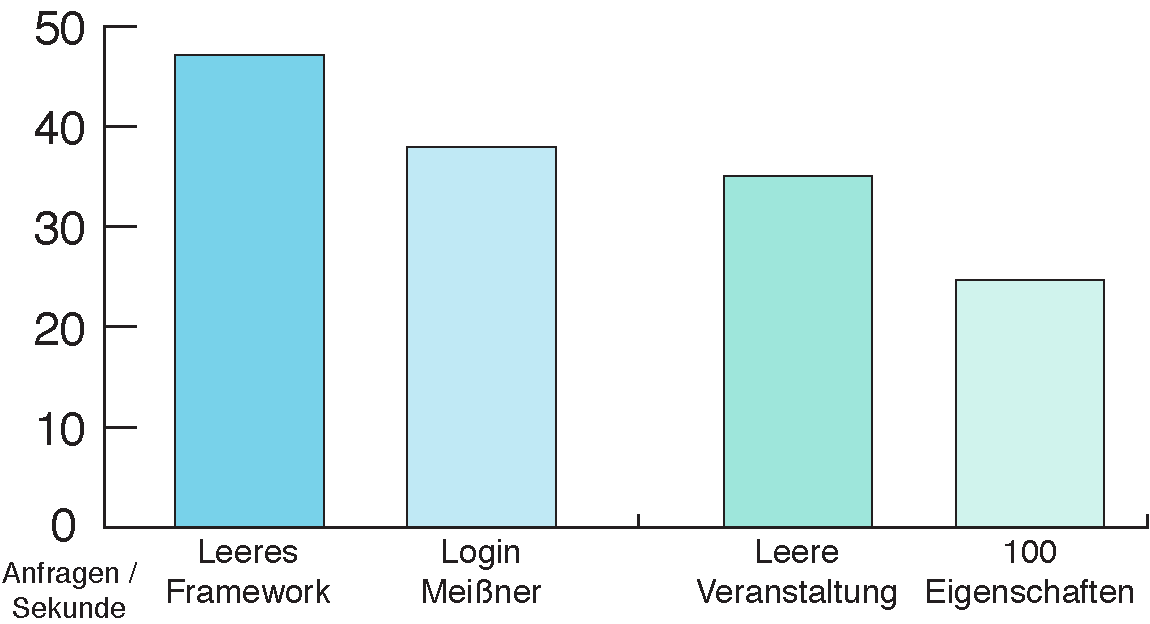
\includegraphics[width=0.7\textwidth]{fig/statistiken_ab.pdf}
	\end{figure}
	\begin{itemize}
		\item Apache Bench: 1000 Verbindungen, immer 10 gleichzeitig
		\item Praxis: Weniger Anfragen nötig durch Offline Cache
	\end{itemize}
\end{frame}

\begin{frame}{WebSocket Server}{Netzwerkauslastung}
	\begin{itemize}
		\item WebSockets: nur 2 Bytes Overhead!
		\item Normale HTTP Anfragen (Polling o.Ä.): 700-800 Bytes Overhead
		\item Besonders relevant bei hoher Anzahl von Clients\pause, bspw. 1.000 Clients:
		\item[]
	\end{itemize}

	\renewcommand{\arraystretch}{1.4}
	\centering
	\begin{tabular}{c|c|c}
		\textbf{Polling} & \textbf{WebSockets} & Einheit\\
		\hline
		800.000 &  2.000 & $\frac{Bytes}{Sekunde}$\\
		6.400.000 &  16.000 & $\frac{Bits}{Sekunde}$\\
		{\color{red}\textbf{6,104} :-(} & {\color{blue}\textbf{0,015} :-)} & $\frac{MBit}{Sekunde}$\\
	\end{tabular}

	\begin{itemize}
		\item[]
		\item[$\Rightarrow$] {\color{red}\textbf{Ersparnis von 400\% Traffic}}
	\end{itemize}
\end{frame}

\begin{frame}{Besonderheiten der Webanwendung}
	\begin{itemize}
		\item Eigenständig lauffähige Webanwendung
		\item Echtzeitaktualisierung
		\item Unterstützung von mobilen Geräten
		\begin{itemize}
			\item Offline Cache!
		\end{itemize}
		\item Automatisches Installationsskript für debianbasierte Systeme
		\item Für die Nutzung im Freien ausgelegt
		\item Modular aufgebaut
		\item Ähnliche Produkte kosten mehrere hundert Dollar und sind meistens nur als Erweiterung für WordPress verfügbar
	\end{itemize}
\end{frame}

  \appendix

  % % % % % % % % % % Ende der eingefügten LaTeX-Dateien % % % % % % % % % %

\end{document}

%
% Hier endet das Dokument
%